\documentclass{beamer}
% \documentclass[handout]{beamer}
% \setbeameroption{show notes}

% You should have already started to think about your talk to the upcoming seminar. So, here are some guidelines that should be applied to the agenda of your presentation:
% 
% #1 Introduction / Context
% #2 Case study
% #3 State-of-the-Art (e.g., papers for PhD students / tools for Engineers)
% #4 Problems / Limitations
% #5 Contribution(s)
% #6 Experimental methodology (<== don't take it easy! )
% #7 Evaluation / Validation
% #8 Perspectives
% #9 Conclusion
% #10 Contribution to LEDA
% 
% 
% For parts #1 to #9, we expect a fair distribution of the slides among the topics, while taking into account your progress (e.g., a 3rd year PhD student should report on a strong Evaluation / Validation, while a 1st year PhD student is more expected to provide a clear view on the state-of-the-art and the foreseen contribution(s) ). We highly recommend you to have a look to last year feedback made by Jacques and Ernesto [1] on the quality of your presentation and their weaknesses.
% 
% For part #10, we expect you to think about how your work can integrate in the LEDA laboratory. If you do not know what LEDA is about, ask Gwen. Gwen has kindly prepared a short document (attached) that summarises the availability of devices in LEDA and the way they are already integrated. This part (as the others) is mandatory and you are expected to propose something valuable for the group.

\usecolortheme[named=blue]{structure}

\mode<presentation>
{
  \usetheme{Warsaw}
  \setbeamercovered{transparent}
}
\title
  [SemFix: Program Repair via Semantic Analysis]
  {SemFix:~Program~Repair~via~Semantic~Analysis}
\author[DeMarco]{Favio~DeMarco}
\institute[U.B.A. - INRIA]{Universidad de Buenos Aires - INRIA}
\date[08/28/2013]{August 28th, 2013}
\subject{Computational Sciences}

% Programming today is a race between software engineers striving to build bigger and better idiot-proof programs, and the Universe trying to produce bigger and better idiots. So far, the Universe is winning.
% Rick Cook, The Wizardry Compiled

\begin{document}

\frame
  {
    \titlepage
  }
%-----------------------------------------------------------------------------80
  \section*{Outline}
%-----------------------------------------------------------------------------80
  \frame
  {
    \frametitle{Outline of Topics}

    \tableofcontents
  }

{
\usebackgroundtemplate{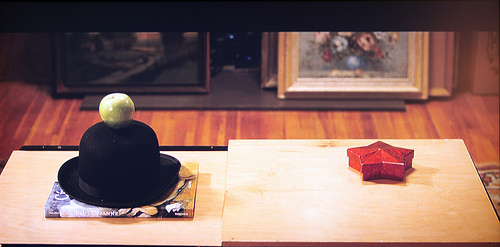
\includegraphics[width=\paperwidth]{500daysofsummer}}%
  \frame
  {
    \frametitle{State of the art}
  }
}

  \frame
  {
    \frametitle{Semfix}
	\Huge Let there be boxes!
	\note{An automated repair method based on symbolic execution, constraint solving and program synthesis. Semfix tries to fix a bug using symbolic execution, an SMT solver and program synthesis.}
  }

\end{document}
